%%%%%%%%%%%%%%%%%%%%%%%%%%%%%%%%%%%%%%%%%
% Beamer Presentation
% LaTeX Template
% Version 1.0 (10/11/12)
%
% This template has been downloaded from:
% http://www.LaTeXTemplates.com
%
% License:
% CC BY-NC-SA 3.0 (http://creativecommons.org/licenses/by-nc-sa/3.0/)
%
%%%%%%%%%%%%%%%%%%%%%%%%%%%%%%%%%%%%%%%%%

%----------------------------------------------------------------------------------------
%	PACKAGES AND THEMES
%----------------------------------------------------------------------------------------

\documentclass[9pt]{beamer}
\usepackage{CJK}
\usepackage{ctex}
\usepackage{graphicx}
\usepackage{subfigure}
\usepackage{longtable}
\usepackage{rotating}
\usepackage{multirow}
\usepackage{algorithm}
\usepackage{algorithmic}
\usepackage{mathtools}
\usepackage{animate}
\usepackage{array}
%\usepackage{media9}
%% A LATEX package for embedding interactive Adobe Flash (SWF) and 3D files (Adobe U3D & PRC) as well as video and sound files or streams (FLV, MP4/H.246, MP3) into PDF documents with Adobe Reader-9/X
%compatibility.
\renewcommand{\algorithmicrequire}{\textbf{Input:}}   %Use Input in the format of Algorithm
\renewcommand{\algorithmicensure}{\textbf{Output:}}  %UseOutput in the format of Algorithm
\newcommand{\e}[1]{\ensuremath{\times 10^{#1}}}
%\mode<presentation>{\usetheme{Madrid}}

\mode<presentation> {

% The Beamer class comes with a number of default slide themes
% which change the colors and layouts of slides. Below this is a list
% of all the themes, uncomment each in turn to see what they look like.

%\usetheme{default}
%\usetheme{AnnArbor}
%\usetheme{Antibes}
%\usetheme{Bergen}
%\usetheme{Berkeley}
%\usetheme{Berlin}
%\usetheme{Boadilla}
%\usetheme{CambridgeUS}
%\usetheme{Copenhagen}
%\usetheme{Darmstadt}
%\usetheme{Dresden}
%\usetheme{Frankfurt}
%\usetheme{Goettingen}
%\usetheme{Hannover}
%\usetheme{Ilmenau}
%\usetheme{JuanLesPins}
%\usetheme{Luebeck}
\usetheme{Madrid}
%\usetheme{Malmoe}
%\usetheme{Marburg}
%\usetheme{Montpellier}
%\usetheme{PaloAlto}
%\usetheme{Pittsburgh}
%\usetheme{Rochester}
%\usetheme{Singapore}
%\usetheme{Szeged}
%\usetheme{Warsaw}

% As well as themes, the Beamer class has a number of color themes
% for any slide theme. Uncomment each of these in turn to see how it
% changes the colors of your current slide theme.

%\usecolortheme{albatross}
\usecolortheme{beaver}
%\usecolortheme{beetle}
%\usecolortheme{crane}
%\usecolortheme{dolphin}
%\usecolortheme{dove}
%\usecolortheme{fly}
%\usecolortheme{lily}
%\usecolortheme{orchid}
%\usecolortheme{rose}
%\usecolortheme{seagull}
%\usecolortheme{seahorse}
%\usecolortheme{whale}
%\usecolortheme{wolverine}

%\setbeamertemplate{footline} % To remove the footer line in all slides uncomment this line
%\setbeamertemplate{footline}[page number] % To replace the footer line in all slides with a simple slide count uncomment this line

%\setbeamertemplate{navigation symbols}{} % To remove the navigation symbols from the bottom of all slides uncomment this line
}

\usepackage{graphicx} % Allows including images
\usepackage{booktabs} % Allows the use of \toprule, \midrule and \bottomrule in tables

\usepackage{color}
%\textcolor{red/blue/green/black/white/cyan/magenta/yellow}{text}

\begin{document}
\begin{CJK*}{GBK}{kai}
%----------------------------------------------------------------------------------------
%	TITLE PAGE
%----------------------------------------------------------------------------------------

\title[Machine Learning]{LN14. ~~Kernels} % The short title appears at the bottom of every slide, the full title is only on the title page

\author{Kun He (����)} % Your name
%\logo{%
%   
\includegraphics[scale=.2]{logo.pdf}\hspace*{4.75cm}~%
%   
\includegraphics[scale=.2]{logo.jpg}\hspace*{0.75cm}%
%   }
%\pgfdeclareimage[width=1cm]{hust}{logo.pdf}
%\logo{\pgfuseimage{hust}{\vspace{-10pt}}}
\titlegraphic{
\includegraphics[width=1.3cm]{logo.pdf}}
\institute[JHL, HUST] % Your institution as it will appear on the bottom of every slide, may be shorthand to save space
{
	Data Mining and Machine Learning Lab\\
	(John Hopcroft Lab)\\
	Huazhong University of Science \& Technology \\ % Your institution for the title page
	\medskip
	\textit{brooklet60@hust.edu.cn} % Your email address
}

\date{2022��5��} % Date, can be changed to a custom date
%====================================================
\frame{\titlepage}

\frame{\frametitle{Table of Contents}\tableofcontents}

\AtBeginSection[]
{
	\begin{frame}{Table of Contents}
		\tableofcontents[currentsection]
	\end{frame}
}


%------------------------------------------------
%------------------------------------------------
\section{Feature Expansion}
%------------------------------------------------
\subsection{Motivation}
\begin{frame}
	\frametitle{Motivation}
	\begin{block}{Motivation}
		\begin{itemize}
			\item
			Linear classifiers are great, but what if there exists no linear decision boundary?
			\item
			As it turns out, there is an elegant way to incorporate non-linearities into most linear classifiers.
		\end{itemize}
	\end{block}
\end{frame}

\subsection{Handcrafted Feature Expansion}
\begin{frame}
	\frametitle{Handcrafted Feature Expansion}
	\begin{itemize}
	\item We can make linear classifiers non-linear by applying basis function (feature transformations) on the input feature vectors. \\
	\item Formally, for a data vector $\mathbf{x}\in\mathbb{R}^d$, we apply the transformation $\mathbf{x} \rightarrow \phi(\mathbf{x})$ where $\phi(\mathbf{x})\in\mathbb{R}^D$. Usually $D \gg d$ because we add dimensions that capture non-linear interactions among the original features.
	\end{itemize}
	\begin{figure}[h]
	\centering		
	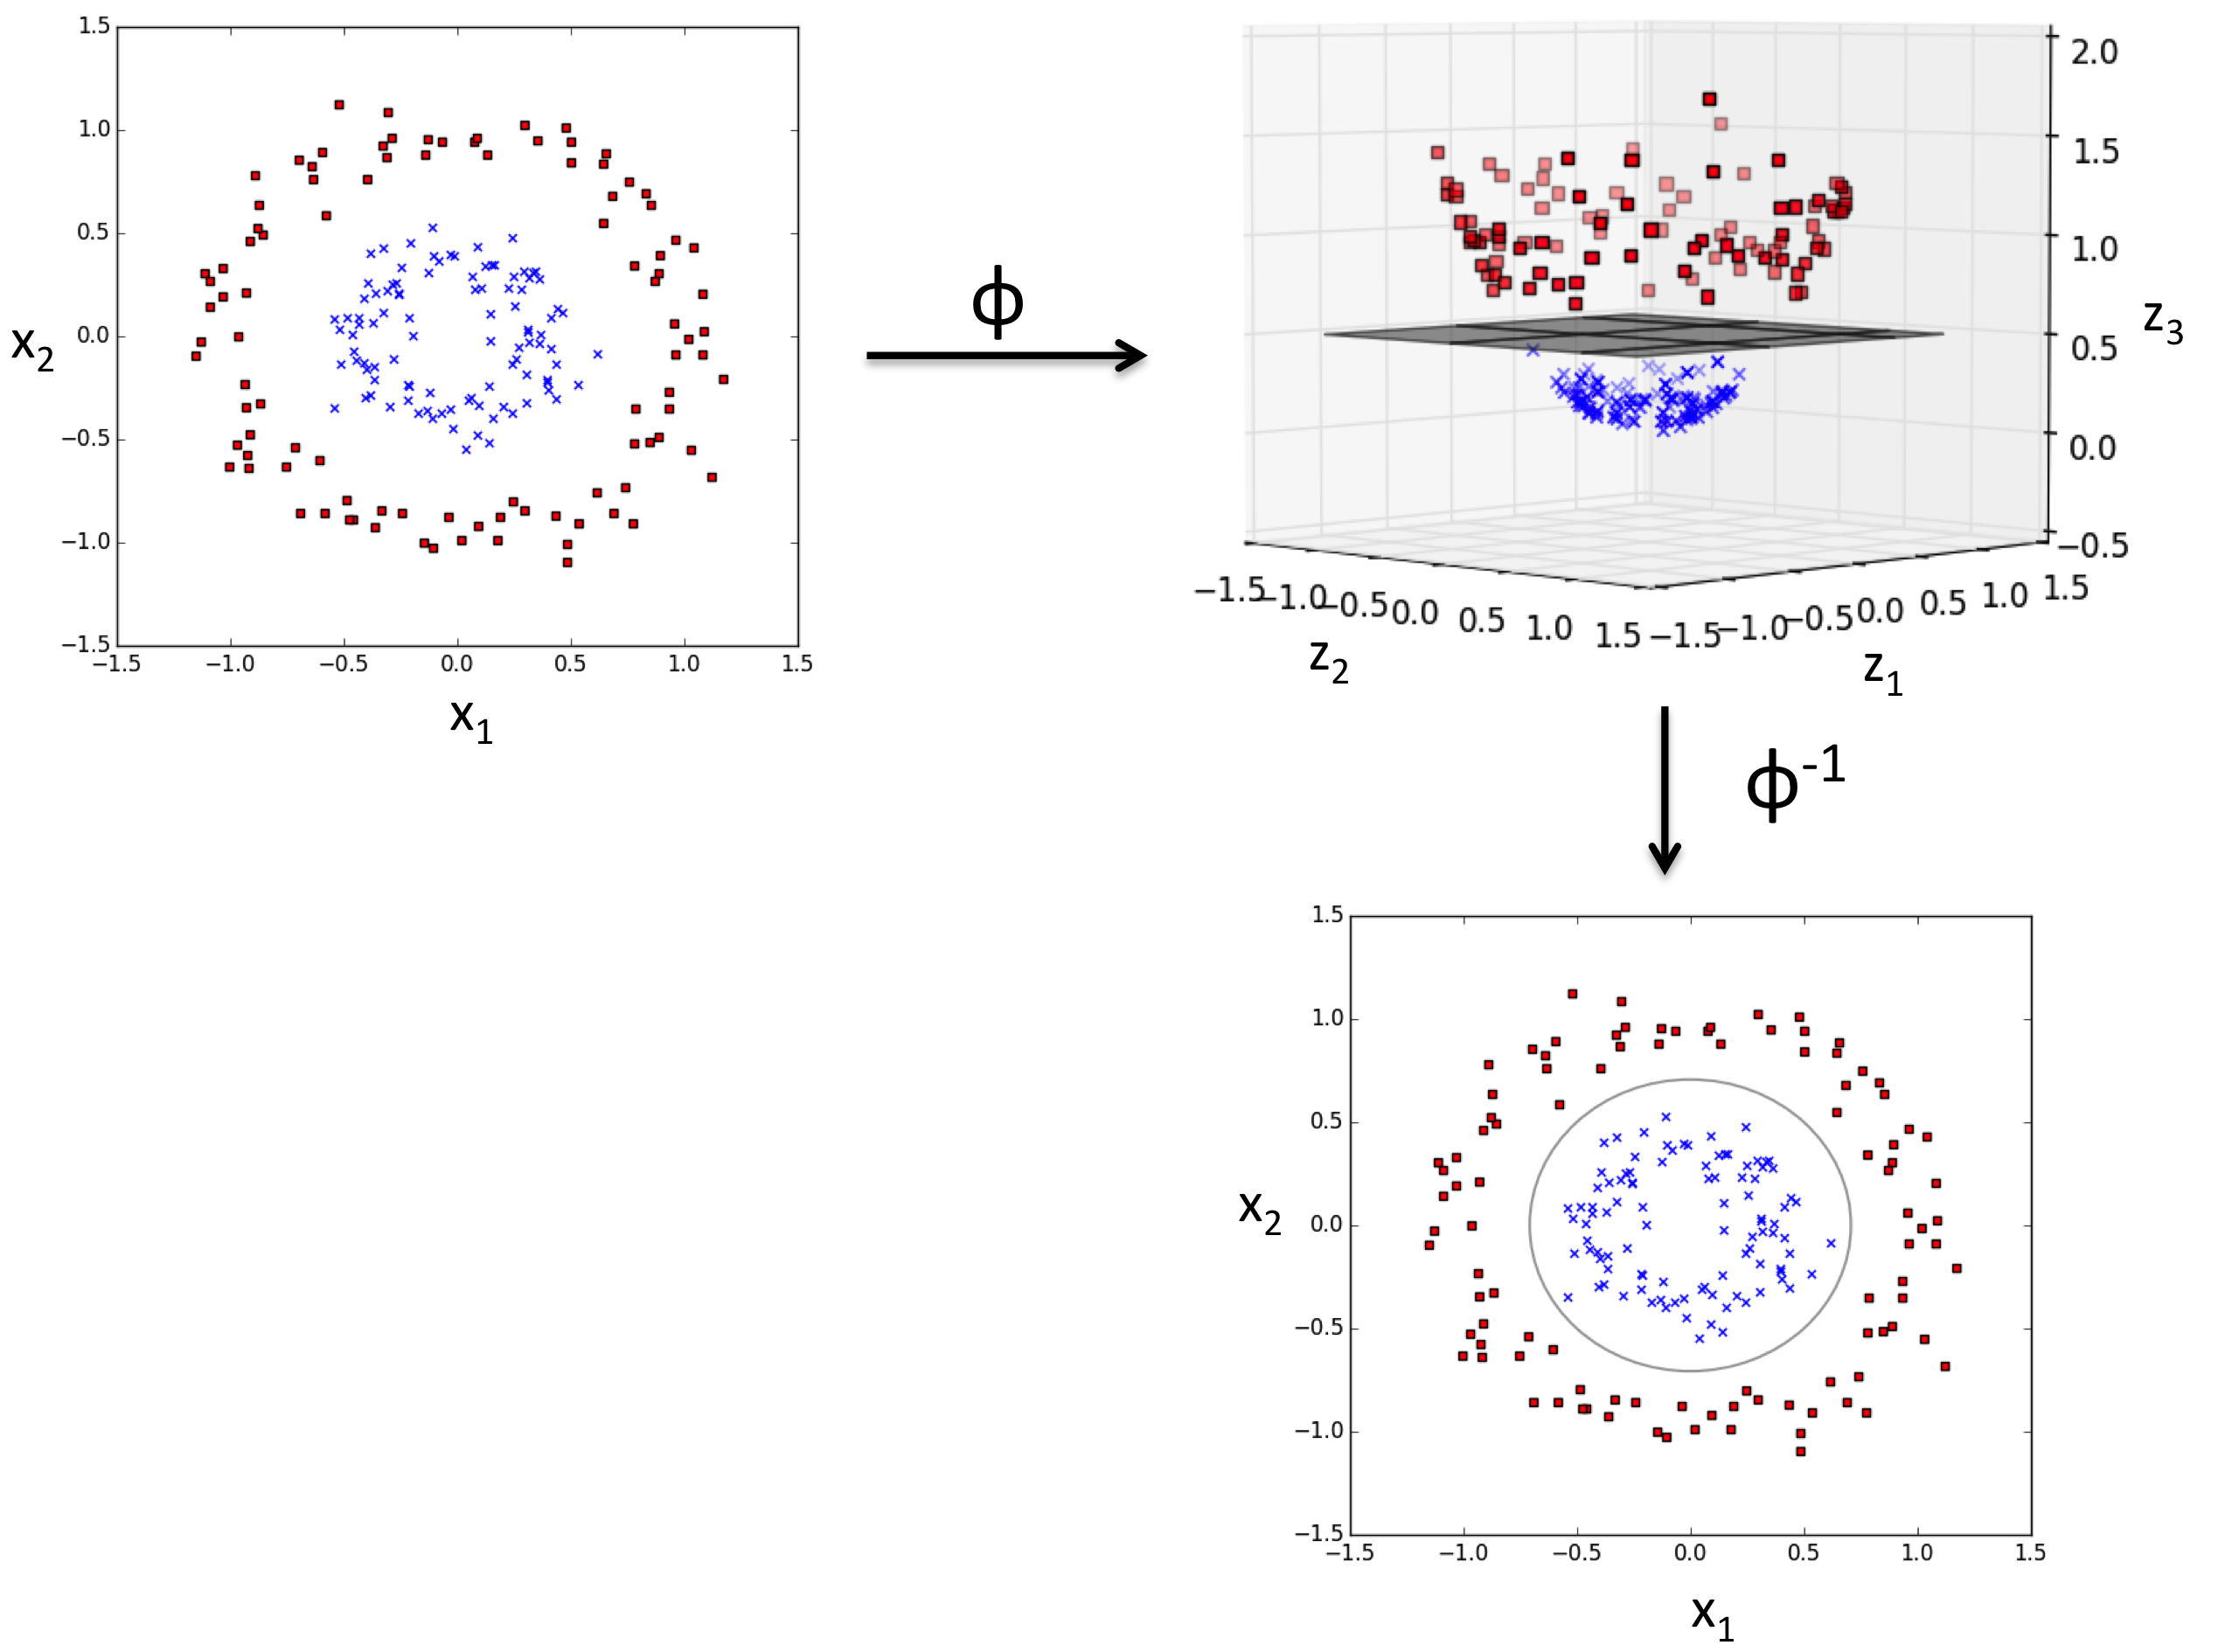
\includegraphics[scale=0.1]{pics/KernelMapping} 		
	\end{figure}
\end{frame}

\begin{frame}
	\frametitle{Handcrafted Feature Expansion}
\begin{block}{Advantage}
	It is simple, and your problem stays convex and well behaved. (i.e. you can still use your original gradient descent code, just with the higher dimensional representation)
\end{block}

\begin{block}{Disadvantage}
	$\phi(\mathbf{x})$ might be very high dimensional.
\end{block}	
	
\end{frame}



\begin{frame}{An Example of Handcrafted Feature Expansion}
	
	Consider the following example: $\mathbf{x}=\begin{pmatrix}x_1\\ x_2\\ \vdots \\ x_d \end{pmatrix}$, and define $\phi(\mathbf{x})=\begin{pmatrix}1\\ x_1\\ \vdots \\x_d \\ x_1x_2 \\ \vdots \\ x_{d-1}x_d\\ \vdots \\x_1x_2\cdots x_d \end{pmatrix}$
	
	\begin{block}{Quiz}
	What is the dimensionality of $\phi(\mathbf{x})$?
	\end{block}	
\end{frame}



\begin{frame}{An Example of Handcrafted Feature Expansion}
	\begin{itemize}
	\item RE: The dimensionality of $\phi(\mathbf{x})$ is $2^d$. 
	\item 	
	This new representation, $\phi(\mathbf{x})$, is very expressive and allows for complicated non-linear decision boundaries - but the dimensionality is extremely high. This makes our algorithm unbearable  slow.
	\end{itemize}	
\end{frame}


\section{The Kernel Trick}
\subsection{The Kernel Trick}
\begin{frame}{The Kernel Trick}
	The kernel trick is a way to get around this dilemma by learning a function in the much higher dimensional space, without ever computing a single vector $\phi(\mathbf{x})$ or ever computing the full vector $\mathbf{w}$. \\~~~\\
	It is a little magical.  
	%It is based on the following observation: 
\begin{block}{Observation}
	If we use gradient descent with any one of our standard loss functions, 
	\textcolor{magenta}{the gradient is a linear combination of the input samples}.
\end{block}	  
\end{frame}


\subsection{Gradient Descent with Squared Loss}
\begin{frame}{Revisiting Gradient Descent with Squared Loss}
	For example, let us take a look at the squared loss:
	\begin{equation*}
	\ell(\mathbf{w}) = \sum_{i=1}^n (\mathbf{w}^\top  \mathbf{x}_i-y_i)^2\label{eq:c15:sql}
	\end{equation*}
	The gradient descent rule, with step-size/learning-rate $s>0$ (we denoted this as $\alpha>0$ in our previous lectures), updates $\mathbf{w}$ over time,
	\begin{equation*}
	w_{t+1} \leftarrow w_t - s(\frac{\partial \ell}{\partial \mathbf{w}})\ \textrm{ where: }
	\frac{\partial \ell}{\partial \mathbf{w}}=\sum_{i=1}^n \underbrace{2(\mathbf{w}^\top  \mathbf{x}_i-y_i)}_{\gamma_i\ :\ \textrm{function of $\mathbf{x}_i, y_i$}} \mathbf{x}_i = \sum_{i=1}^n\gamma_i \mathbf{x}_i
	\end{equation*}
	We will now show that we can express $\mathbf{w}$ as a \textbf{linear combination of all input vectors},
	\begin{equation*}
	\mathbf{w}=\sum_{i=1}^n \alpha_i {\mathbf{x}}_i.\label{eq:c15:alphas}
	\end{equation*}    
\end{frame}

 

\begin{frame}{Gradient Descent with Squared Loss}
\begin{block}{Lemma: $\mathbf{w}$ is a linear combination of all input vectors.}
	\begin{equation*}
	\mathbf{w}=\sum_{i=1}^n \alpha_i {\mathbf{x}}_i.\label{eq:c15:alphas}
	\end{equation*}    
\end{block}
	Since the loss is convex, the final solution is independent of the initialization, and we can initialize $\mathbf{w}_0$ to be whatever we want. For convenience, let us pick $\mathbf{w}_0=\begin{pmatrix}0 \\ \vdots \\ 0\end{pmatrix}$. 
	\\ For this initial choice of $\mathbf{w}_0$, the linear combination in $\mathbf{w}=\sum_{i=1}^n \alpha_i {\mathbf{x}}_i$ is trivially: \\ ~~~~~~~~~~~~~~~~~~~~~~~~$\alpha_1=\dots=\alpha_n=0$. 
	
\end{frame}

\begin{frame}{Gradient Descent with Squared Loss}
	We now show that throughout the entire gradient descent optimization such coefficients $\alpha_1,\dots,\alpha_n$ must always exist, as we can re-write the gradient updates entirely in terms of updating the $\alpha_i$ coefficients:
	
	
	\begin{figure}[h]
		\centering
		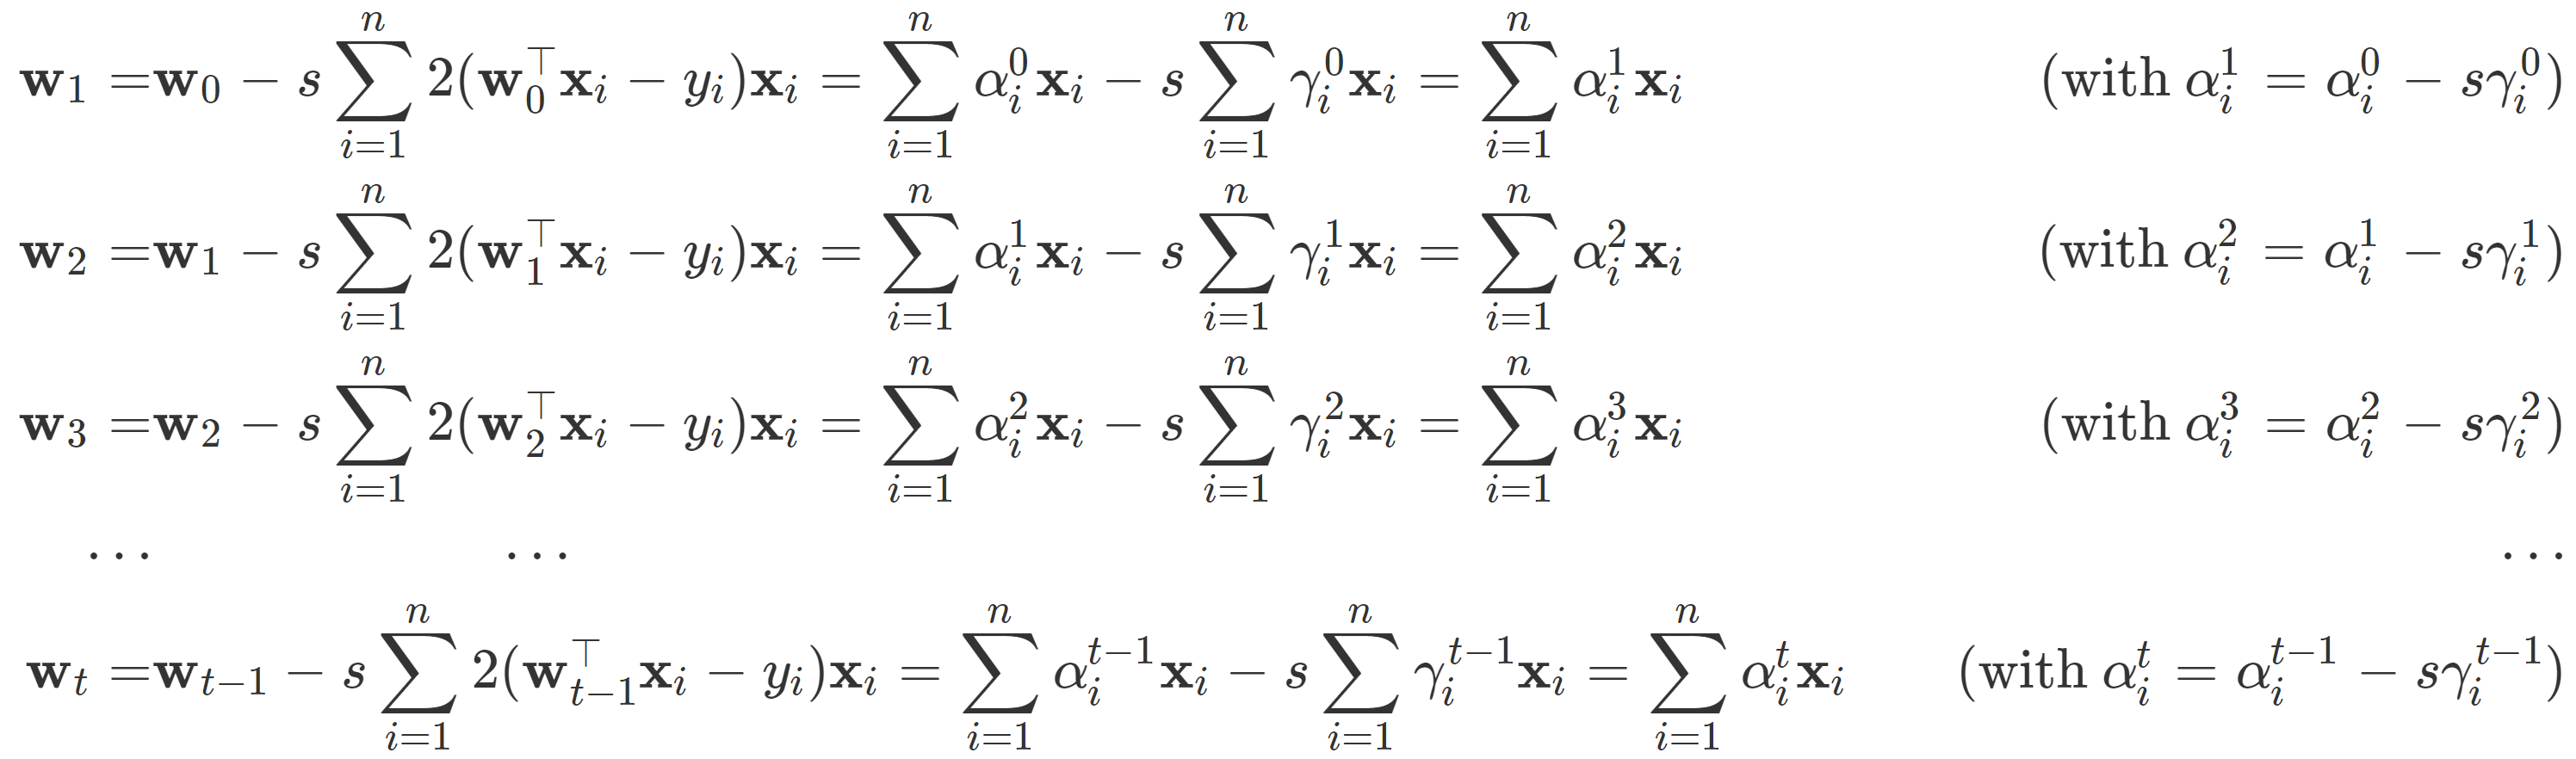
\includegraphics[scale=0.15]{pics/equ.jpg}
	\end{figure}
	%\begin{align*}
	% \mathbf{w}_1=&\mathbf{w}_0-s\sum_{i=1}^n2(\mathbf{w}_0^\top  \mathbf{x}_i-y_i)\mathbf{x}_i\\
	% =&\sum_{i=1}^n \alpha_i^0 {\mathbf{x}}_i-s\sum_{i=1}^n\gamma_i^0\mathbf{x}_i=\sum_{i=1}^n\alpha_i^1\mathbf{x}_i &(\textrm{with $\alpha_i^1=\alpha_i^0-s\gamma_i^0$})\\
	% \mathbf{w}_2=&\mathbf{w}_1-s\sum_{i=1}^n2(\mathbf{w}_1^\top  \mathbf{x}_i-y_i)\mathbf{x}_i\\
	% =&\sum_{i=1}^n \alpha_i^1\mathbf{x}_i-s\sum_{i=1}^n\gamma_i^1\mathbf{x}_i=\sum_{i=1}^n\alpha_i^2\mathbf{x}_i &(\textrm{with $\alpha_i^2=\alpha_i^1\mathbf{x}_i-s\gamma_i^1$})\\
	% \mathbf{w}_3=&\mathbf{w}_2-s\sum_{i=1}^n2(\mathbf{w}_2^\top  \mathbf{x}_i-y_i)\mathbf{x}_i\\
	% =&\sum_{i=1}^n \alpha_i^2\mathbf{x}_i-s\sum_{i=1}^n\gamma_i^2\mathbf{x}_i=\sum_{i=1}^n\alpha_i^3\mathbf{x}_i &(\textrm{with $\alpha_i^3=\alpha_i^2-s\gamma_i^2$})\\
	% \cdots & \qquad\qquad\qquad\cdots &\cdots\\
	% \mathbf{w}_t=&\mathbf{w}_{t-1}-s\sum_{i=1}^n2(\mathbf{w}_{t-1}^\top  \mathbf{x}_i-y_i)\mathbf{x}_i\\
	% =&\sum_{i=1}^n \alpha_i^{t-1}\mathbf{x}_i-s\sum_{i=1}^n\gamma_i^{t-1}\mathbf{x}_i=\sum_{i=1}^n\alpha_i^t\mathbf{x}_i &(\textrm{with $\alpha_i^t=\alpha_i^{t-1}-s\gamma_i^{t-1}$})&
	% \end{align*}
\end{frame}

\begin{frame}{Gradient Descent with Squared Loss}
	\begin{figure}[h]
	\centering
	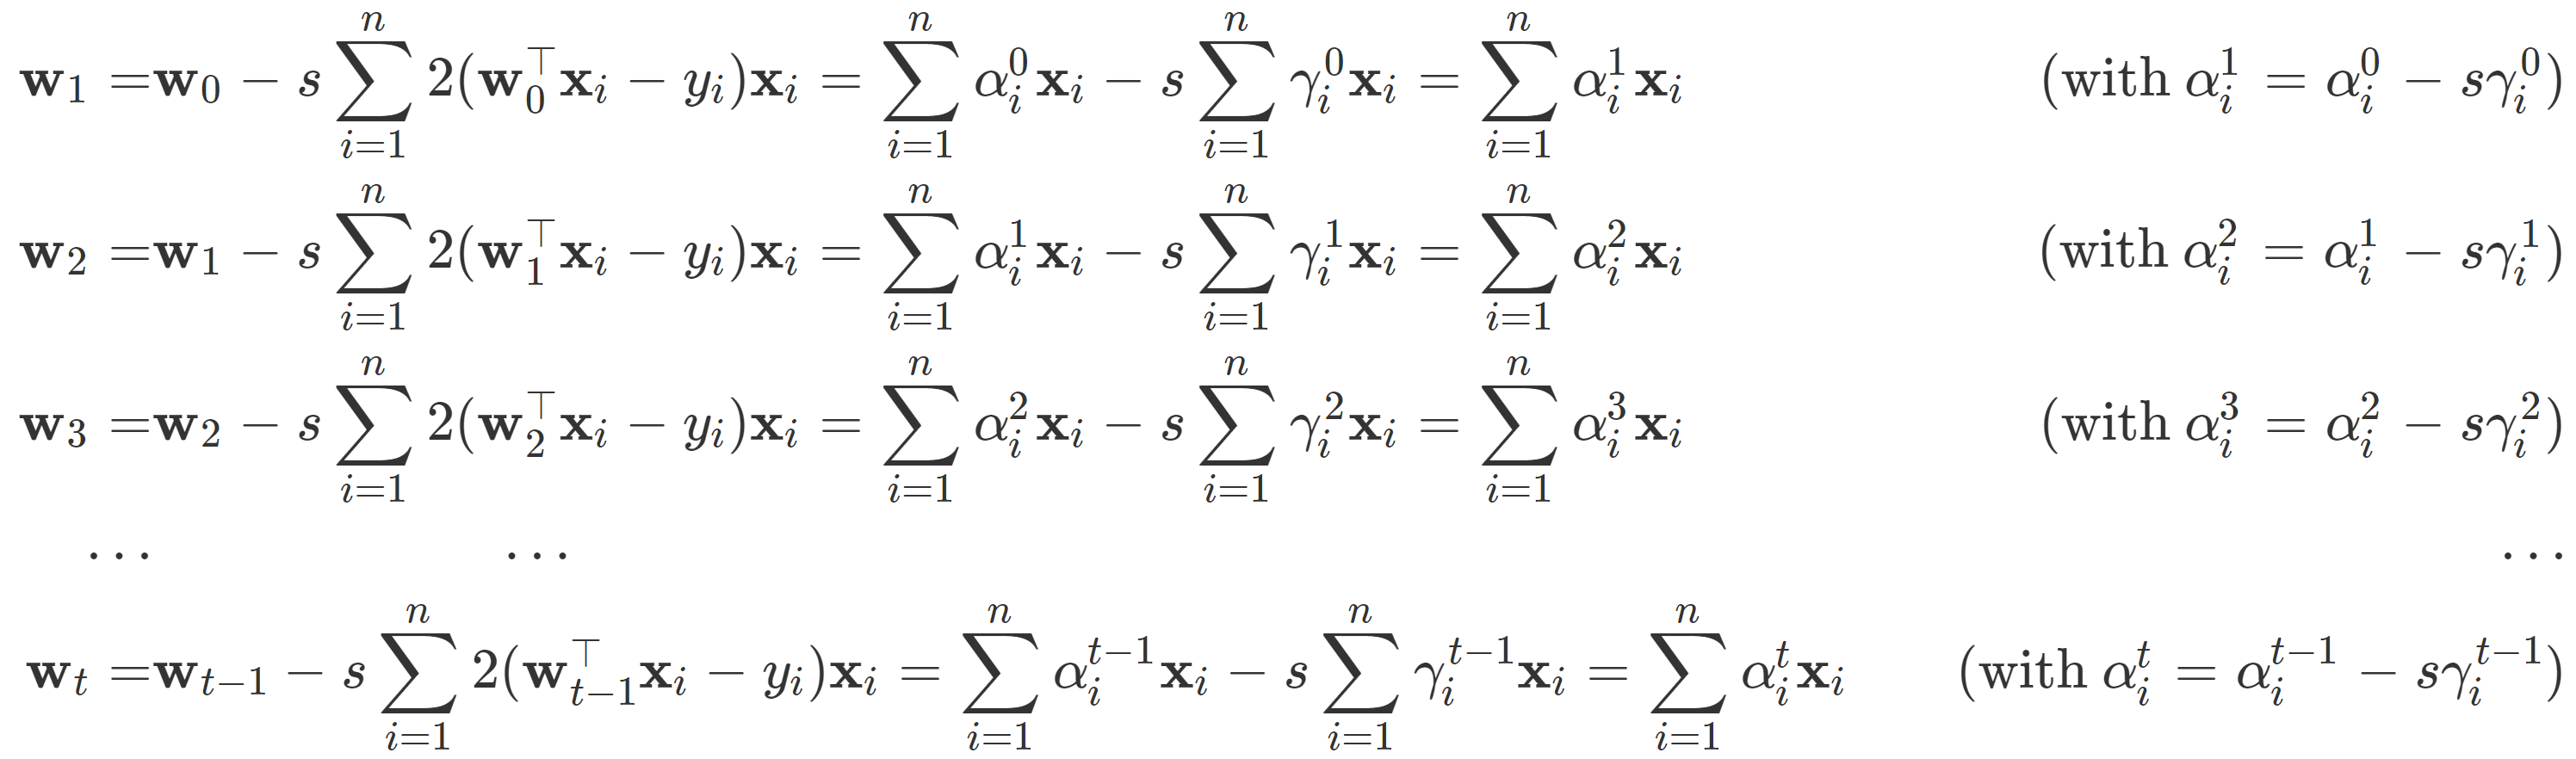
\includegraphics[scale=0.15]{pics/equ.jpg}
	\end{figure}	
	Formally, the argument is by induction. $\mathbf{w}$ is trivially a linear combination of our training vectors for $\mathbf{w}_0$ (base case). If we apply the inductive hypothesis for $\mathbf{w}_t$ it follows for $\mathbf{w}_{t+1}$.
	
	The update-rule for $\alpha_i^t$ is thus
	\begin{equation*}
	\alpha_i^t=\alpha_i^{t-1}-s\gamma_i^{t-1}, \textrm{ and we have } \alpha_i^t=-s\sum_{r=0}^{t-1}\gamma_i^{r}.
	\end{equation*}
\end{frame}

\begin{frame}{Substitution of $\mathbf{w}$}
	\[ \mathbf{w}_t=\sum_{i=1}^n\alpha_i^t\mathbf{x}_i\]
	In other words, we can perform the entire gradient descent update rule without ever expressing $\mathbf{w}$ explicitly. We just keep track of the $n$ coefficients $\alpha_1,\dots,\alpha_n$. \\~~\\
	Now that $\mathbf{w}$ can be written as a linear combination of the training set, we can also express the inner-product of $\mathbf{w}$ with any input ${\mathbf{x}}_i$ purely in terms of inner-products between training inputs:
	\begin{equation*}
	\mathbf{w}^\top {\mathbf{x}}_j=\sum_{i=1}^n \alpha_i {\mathbf{x}}_i^\top{\mathbf{x}}_j.\nonumber
	\end{equation*}
\end{frame}

\begin{frame}{Substitution of $\mathbf{w}$}
	\begin{itemize}
	\item Consequently, we can also re-write the squared-loss from $\ell(\mathbf{w}) = \sum_{i=1}^n (\mathbf{w}^\top \mathbf{x}_i-y_i)^2$ entirely in terms of inner-product between training inputs:
	\end{itemize}
	\begin{equation*}
	\ell(\mathbf{\alpha}) = \sum_{i=1}^n \left(\sum_{j=1}^n\alpha_j\mathbf{x}_j^\top  \mathbf{x}_i-y_i\right)^2\label{eq:c15:sql:ip} 
	\end{equation*}

	\begin{itemize}
	\item During test-time we also only need these coefficients to make a prediction on a test-input $x_t$, and can write the entire classifier in terms of inner-products between the test point and training points:
	\end{itemize}
\begin{equation*}
h({\mathbf{x}}_t)=\mathbf{w}^\top {\mathbf{x}}_t=\sum_{j=1}^n\alpha_j{\mathbf{x}}_j^\top {\mathbf{x}}_t.
\end{equation*}	
\end{frame}

 

\begin{frame}{Substitution of $\mathbf{w}$}
	\begin{itemize}
	\item During test-time, for a test-input $x_t$, we have:
	\end{itemize}
	\begin{equation*}
	h({\mathbf{x}}_t)=\mathbf{w}^\top {\mathbf{x}}_t=\sum_{j=1}^n\alpha_j{\mathbf{x}}_j^\top {\mathbf{x}}_t.
	\end{equation*}	
	
	\begin{block}{Do you notice a theme?}
		The only information we ever need in order to learn a hyper-plane classifier with the squared-loss is \textbf{inner-products between all pairs of data vectors.}
	\end{block}
\end{frame}
 

\subsection{Inner-Product Computation}
\begin{frame}{Inner-Product Computation}
	Let's go back to the previous example, $\phi(\mathbf{x})=\begin{pmatrix}1\\ x_1\\ \vdots \\x_d \\ x_1x_2 \\ \vdots \\ x_{d-1}x_d\\ \vdots \\x_1x_2\cdots x_d \end{pmatrix}$.
	
	The inner product $\phi(\mathbf{x})^\top \phi(\mathbf{z})$ can be formulated as:
	\begin{equation*}
	\phi(\mathbf{x})^\top \phi(\mathbf{z})=1\cdot 1+x_1z_1+x_2z_2+\cdots +x_1x_2z_1z_2+ \cdots +x_1\cdots x_dz_1\cdots z_d=\prod_{k=1}^d(1+x_kz_k)\text{.}\label{eq:c15:poly}
	\end{equation*}
	The sum of $2^d$ terms becomes the product of $d$ terms. We can compute the inner-product from the above formula in time $O(d)$ instead of $O(2^d)$! 
\end{frame}

\begin{frame}{Inner-Product Computation}
	We define the function
	\begin{equation*}
	\underbrace{\mathsf{k}(\mathbf{x}_i,\mathbf{x}_j)}_{\text{this is called the} \textbf{ kernel function}}=\phi(\mathbf{x}_i)^\top \phi(\mathbf{x}_j).
	\end{equation*}
	With a finite training set of $n$ samples, inner products are often pre-computed and stored in a Kernel Matrix:
	\begin{equation*}
	\mathsf{K}_{ij}=\phi(\mathbf{x}_i)^\top \phi(\mathbf{x}_j).
	\end{equation*}
	If we store the matrix $\mathsf{K}$, we only need to do simple inner-product look-ups and low-dimensional computations throughout the gradient descent algorithm. \\~~\\
	The final classifier becomes:

	\[
	h(\mathbf{x}_t)=\sum_{j=1}^n\alpha_j\mathsf{k}(\mathbf{x}_j,\mathbf{x}_t).
	\]

\end{frame}

\begin{frame}{From $O(2^d)$ to $O(n^2)$}
	Recall:
	\begin{equation*}
	\ell(\mathbf{w}) = \sum_{i=1}^n (\mathbf{w}^\top  \mathbf{x}_i-y_i)^2\label{eq:c15:sql}
	\end{equation*}
\begin{equation*}
w_{t+1} \leftarrow w_t - s(\frac{\partial \ell}{\partial \mathbf{w}})\ \textrm{ where: }
\frac{\partial \ell}{\partial \mathbf{w}}=\sum_{i=1}^n \underbrace{2(\mathbf{w}^\top  \mathbf{x}_i-y_i)}_{\gamma_i\ :\ \textrm{function of $\mathbf{x}_i, y_i$}} \mathbf{x}_i = \sum_{i=1}^n\gamma_i \mathbf{x}_i
\end{equation*}	
	\\
	During training in the new high dimensional space of $\phi(\mathbf{x})$ we want to compute $\gamma_i$ through kernels, without ever computing any $\phi(\mathbf{x}_i)$ or even $\mathbf{w}$. We previously established that $\mathbf{w}=\sum_{j=1}^n\alpha_j \phi(\mathbf{x}_j)$, and $\gamma_i=2(\mathbf{w}^\top \phi(\mathbf{x}_i)-y_i)$. 
	\\~~\\
	It follows that $\gamma_i=2(\sum_{j=1}^n \alpha_jK_{ij})-y_i)$. The gradient update in iteration $t+1$ becomes:
	\[ \alpha_i^{t+1}\leftarrow \alpha_i^t-2s(\sum_{j=1}^n \alpha_j^tK_{ij})-y_i).\]
	\\
	
	As we have $n$ such updates to do, the amount of work per gradient update in the transformed space is $O(n^2)$ --- far better than $O(2^d)$.
\end{frame}


\section{General Kernels}
\subsection{Popular Kernel Functions}
\begin{frame}{Popular Kernel Functions}
	Below are some popular kernel functions:
	\begin{itemize}
		\item 
		\textbf{Linear}: $\mathsf{K}(\mathbf{x},\mathbf{z})=\mathbf{x}^\top \mathbf{z}$.\\
		(The linear kernel is equivalent to just using a good old linear classifier - but it can be faster to use a kernel matrix if the dimensionality $d$ of the data is high.)
		\item
		\textbf{Polynomial}: $\mathsf{K}(\mathbf{x},\mathbf{z})=(1+\mathbf{x}^\top \mathbf{z})^d$.
		\item
		\textbf{Radial Basis Function (RBF) (aka Gaussian Kernel)}: $\mathsf{K}(\mathbf{x},\mathbf{z})= e^\frac{-\|\mathbf{x}-\mathbf{z}\|^2}{\sigma^2}$.\\
		The RBF kernel is the most popular Kernel! It is a Universal approximator!! Its corresponding feature vector is infinite dimensional and cannot be computed. However, very effective low dimensional approximations exist (see \href{https://people.eecs.berkeley.edu/~brecht/papers/08.rah.rec.nips.pdf}{this paper}).
		\item
		\textbf{Exponential Kernel}: $\mathsf{K}(\mathbf{x},\mathbf{z})= e^\frac{-\| \mathbf{x}-\mathbf{z}\|}{2\sigma^2}$
		\item
		\textbf{Laplacian Kernel}: $\mathsf{K}(\mathbf{x},\mathbf{z})= e^\frac{-| \mathbf{x}-\mathbf{z}|}{\sigma}$
		\item
		\textbf{Sigmoid Kernel}: $\mathsf{K}(\mathbf{x},\mathbf{z})=\tanh(\mathbf{a}\mathbf{x}^\top + c)$,
		$\tanh(x) = \frac{e^x-e^{-x}}{e^x +e^{-x}}$
	\end{itemize}
\end{frame}

\subsection{Kernel Functions}
\begin{frame}{Kernel Functions}
	\textbf{Q: }Can any function $\mathsf{K}(\cdot,\cdot)\rightarrow{\mathcal{R}}$ be used as a kernel?\\
	\textbf{A: }No, the matrix $\mathsf{K}(\mathbf{x}_i,\mathbf{x}_j)$ has to correspond to real inner-products after some transformation ${\mathbf{x}}\rightarrow \phi({\mathbf{x}})$. This is the case if and only if $\mathsf{K}$ is positive semi-definite.
	\begin{block}{Definition of Positive Semi-definite}
		A matrix $A\in \mathbb{R}^{n\times n}$ is positive semi-definite iff $\forall \mathbf{q}\in\mathbb{R}^n, \mathbf{q}^\top A\mathbf{q}\geq 0$.
	\end{block}
\end{frame}

\begin{frame}{Kernel Functions}
	Remember $\mathsf{K}_{ij}=\phi(\mathbf{x}_i)^\top \phi(\mathbf{x}_j)$. So $\mathsf{K}=\Phi^\top\Phi$, where $\Phi=[\phi(\mathbf{x}_1),\dots,\phi(\mathbf{x}_n)]$. 
	\\
	It follows that $\mathsf{K}$ is p.s.d., because $\mathbf{q}^\top\mathsf{K}\mathbf{q}=(\Phi^\top \mathbf{q})^2\geq 0$. 
	\\~~~\\
	Inversely, if any matrix $\mathbf{A}$ is p.s.d., it can be decomposed as $A=\Phi^\top\Phi$ for some realization of $\Phi$.
	\\~~~\\
	You can even define kernels over sets, strings, graphs and molecules.
\end{frame}

\begin{frame}{Example: RBF Kernel}
	\begin{figure}
		\centering
		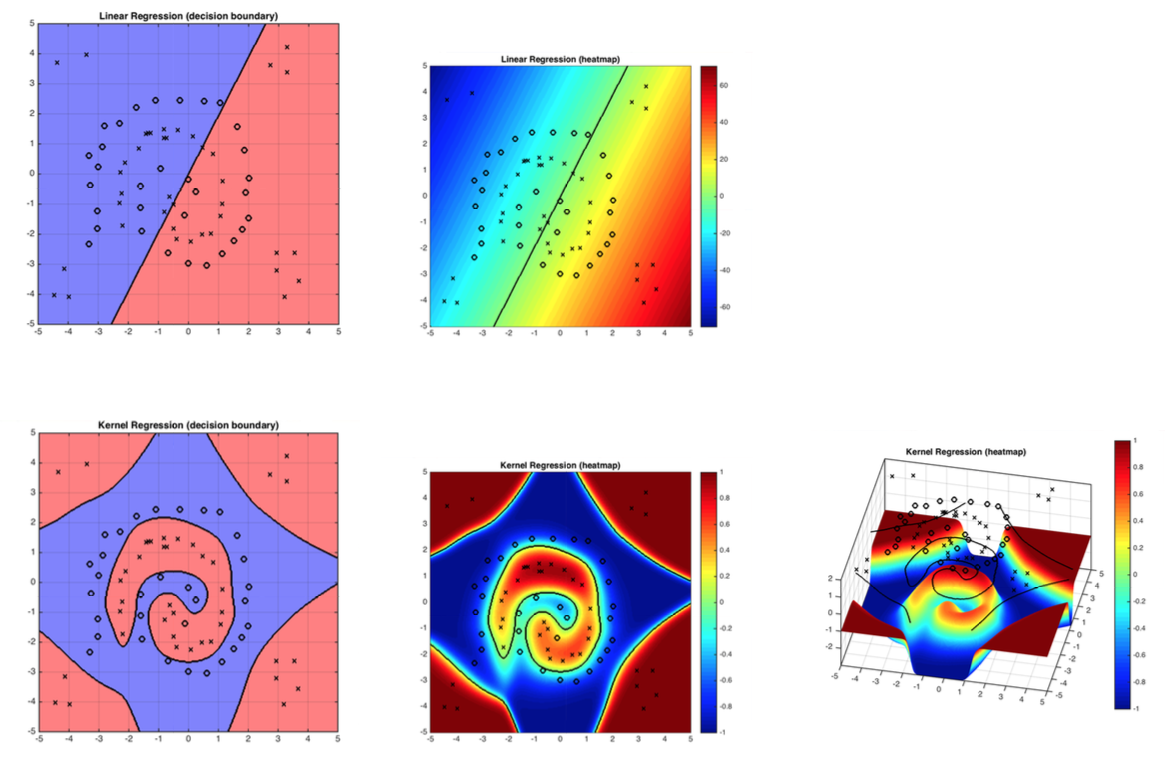
\includegraphics[scale=0.32]{pics/kernel.png}
	\end{figure}
	The demo shows how kernel function solves the problem linear classifiers can not solve. RBF works well with the decision boundary in this case.
\end{frame}



\begin{frame}
\Huge{\centerline{The End}}
\end{frame}
\end{CJK*}
\end{document}
%\end{document}
